\documentclass[a4paper,11pt]{article}

\usepackage[utf8]{inputenc}
\usepackage{adjustbox}
\usepackage[italian]{babel}
\usepackage[T1]{fontenc}
\usepackage[a4paper, margin=2.5cm]{geometry}
\usepackage{subcaption} 
\usepackage{float}
\usepackage{tabularx}
\usepackage{booktabs}  
\usepackage{enumitem}
\usepackage{array}
\usepackage{graphicx}
\usepackage{xcolor}      
\usepackage{tabularray}  
\usepackage{textcomp}			 	
\usepackage{titling}			 	
\usepackage{fancyhdr}			 	
\usepackage{lmodern}       
\usepackage{microtype}     
\usepackage{parskip} 
\usepackage{bm}						
\usepackage{caption}				
\usepackage{listings}

\usepackage[normalem]{ulem}
\usepackage{hyperref}
\hypersetup{
	colorlinks=false,  
	pdfborder={0 0 0}   
}

\let\oldhref\href
\renewcommand{\href}[2]{\oldhref{#1}{\uline{#2}}}

% Definizione dello stile per Java
\lstset{
    language=Java,
    basicstyle=\ttfamily\small,
    keywordstyle=\color{blue}\bfseries,
    commentstyle=\color{green!60!black},
    stringstyle=\color{orange},
    numbers=none,                   
    breaklines=true,
    frame=single,
    backgroundcolor={},
    showstringspaces=false,
    escapeinside={(*@}{@*)}      
}

\usepackage[italian]{cleveref}

\pagestyle{fancy}

\graphicspath{{img/}}

\captionsetup{
	justification=centering, 
	font=small
}

\title{Ingegneria del Software \\ \Large SunSpot: Gestionale per la prenotazione digitale di stabilimenti balneari} 
\author{Soldani Leonardo - 7139732 \\ Neamtu Narcis Daniel - 7133414}
\date{Marzo 2026} 

\begin{document}

\makeatletter
\begin{titlepage}
	\centering
	\vspace*{1cm}
	
\includegraphics[width=0.7\textwidth]{img/logoUnifi}
	\vfill
	{\huge \bfseries \@title\par}
	\vfill
	{\Large \@author\par}
	\vspace{2cm}
\end{titlepage}
\makeatother

\newpage

\renewcommand{\contentsname}{Indice}
\tableofcontents
\newpage

\pagestyle{plain}
\setcounter{page}{1}

\section{Introduzione}
Il progetto SunSpot nasce dall'esigenza di digitalizzare e modernizzare il settore degli stabilimenti balneari, un ambito che ancora oggi mostra una certa resistenza all'adozione di piattaforme web integrate.
\newline L'obiettivo principale è fornire un'infrastruttura capace di permettere all'utente di prenotare in modo rapido e intuitivo un ombrellone presso uno dei lidi aderenti al servizio, trasformando la pianificazione di una giornata al mare in un'operazione a portata di click, offrendo al contempo ai gestori uno strumento completo per il controllo della propria attività.

Per garantire un ecosistema sicuro e affidabile, SunSpot integra un sistema di regolazione basato su recensioni verificate e un meccanismo di segnalazione (report) tra utenti e gestori, volto a preservare l'integrità del servizio e a migliorare costantemente l'esperienza d'uso per tutti gli attori coinvolti.

\section{Ambiente e tecnologie utilizzate}
L'applicazione è stata sviluppata utilizzando le seguenti tecnologie:

\subsection{Linguaggio e Tool di Build}
\begin{itemize}
    \item \textbf{Java 25} - Scelto per l'utilizzo delle funzionalità più recenti della JDK.
    \item \textbf{Maven 3.8.5} - Strumento di build e gestione delle dipendenze.
\end{itemize}

\subsection{Database e Persistenza}
\begin{itemize}
    \item \textbf{MySQL 8.3.0} - Database relazionale utilizzato per la persistenza dei dati.
    \item \textbf{MySQL Connector/J} - Driver ufficiale per la gestione della connessione al database.
\end{itemize}

\subsection{Librerie e Containerizzazione}
\begin{itemize}
    \item \textbf{BCrypt 0.10.2} - Utilizzata per l'hashing e la gestione sicura delle password.
    \item \textbf{Docker \& Docker Compose 3.8} - Utilizzati per containerizzare il database MySQL, garantendo un ambiente di esecuzione isolato, persistente e facilmente riproducibile.
\end{itemize}

\subsection{Testing e Analisi}
\begin{itemize}
    \item \textbf{JUnit 5.12.1} - Framework per l'esecuzione dei test unitari.
    \item \textbf{Mockito 5.23.0} - Utilizzato per la simulazione di dipendenze durante i test (mocking).
    \item \textbf{JUnit Platform Suite} - Strumento per l'organizzazione e l'esecuzione dei test.
\end{itemize}

\subsection{Intelligenza artificiale}
A supporto dello sviluppo del progetto sono stati utilizzati i modelli linguistici \textit{Gemini 3} e \textit{Gemini 3.1}. L'impiego di tali strumenti si è concentrato sui seguenti ambiti:
\begin{itemize}
	\item \textbf{Architettura progetto}: una volta definiti gli UML alla base del nostro progetto, abbiamo consultato i modelli per un confronto critico sui pattern architetturali (\autoref{cap:Progettazione}) più idonei al nostro contesto applicativo.
	\item  \textbf{Generazione codice ripetitivo}: al fine di ottimizzare i tempi di sviluppo, l'intelligenza artificiale è stata utilizzata per la generazione di codice strutturale e ripetitivo (es. pattern \textit{Builder}). Ha inoltre fornito spunti per soluzioni alternative in componenti critici, come nel caso del \textit{TransactionManager}. L'utilizzo è sempre stato posto sotto controllo umano al fine di garantire l'integrità del codice e la corretta organizzazione di quest'ultimo.
	\item \textbf{Testing}: i modelli sono stati impiegati come supporto per la stesura dei casi di test e per una verifica finale sulla copertura e completezza della suite di testing, assicurando una maggiore robustezza al software prodotto.
\end{itemize}

\section{Use Cases}

\subsection{Utenti del sistema}

Il programma coinvolge tre attori principali: Customer, Owner e Admin. Ciascuno di essi ha la possibilità di effettuare azioni specifiche per il proprio ruolo:

\begin{itemize}
	\item \textbf{Customer}: utente finale dell'applicazione. Ha la possibilità di effettuare prenotazioni scegliendo l'ombrellone desiderato; può richiedere inoltre servizi extra come lettini, sdraio e sedie, o la prenotazione di un camerino. Questa tipologia di utente può rilasciare un'unica recensione per ogni spiaggia presso cui ha prenotato e può inviare una segnalazione (report) agli admin qualora riscontri violazioni delle linee guida da parte di uno stabilimento.
	\item \textbf{Owner}: gestore dello stabilimento balneare. Ha il compito di configurare il proprio lido partendo dalla segnalazione dei servizi comuni, passando per l'organizzazione geografica della spiaggia in zone con diverse fasce di prezzo, fino alla possibilità di definire stagionalità con diverse tariffe. Può inoltre effettuare un report nei confronti dei customer che hanno tenuto comportamenti scorretti, come ad esempio il mancato rispetto di una prenotazione.
	\item \textbf{Admin}: è colui che svolge il ruolo di gestore dell'ambiente commerciale offerto dall'applicazione, accogliendo i report e valutandoli tramite l'accesso alla cronologia dei report inviati e ricevuti dagli utenti, con la possibilità di accettarli o rifiutarli. Al fine di gestire l'ambiente, l'admin utilizza lo strumento del ban, che può colpire sia i customer che gli owner/spiagge. Il ban può essere di due tipi: da una singola spiaggia (applicabile solo ai customer) oppure dall'intera applicazione (applicabile a entrambi).
\end{itemize}

\newpage

\subsection{Descrizione Use Cases}
Il programma si pone l'obiettivo di implementare un'applicazione a scopi commerciali; di conseguenza l'azione di eliminare prenotazioni, spiagge, utenti ed altre informazioni di natura fiscale risulterebbe un comportamento superficiale da parte dei programmatori. Per questo motivo, il sistema non prevede l'eliminazione fisica di record sensibili, ma utilizza un meccanismo di disattivazione logica.

Di seguito (\autoref{fig:UseCases}) è riportato il diagramma degli Use Cases del progetto, nelle sezioni successive verranno analizzati nel dettaglio i flussi più rilevanti.
\begin{figure}[H] 
    \centering
    \makebox[\textwidth][c]{
        \includegraphics[width=1.15\textwidth]{DiagrammaUseCases.pdf} 
    }
    \caption{Diagramma degli Use Cases}
    \label{fig:UseCases}
\end{figure}

\subsubsection{Manage User Account}

\begin{figure}[H]
    \centering
    \makebox[\textwidth][c]{
        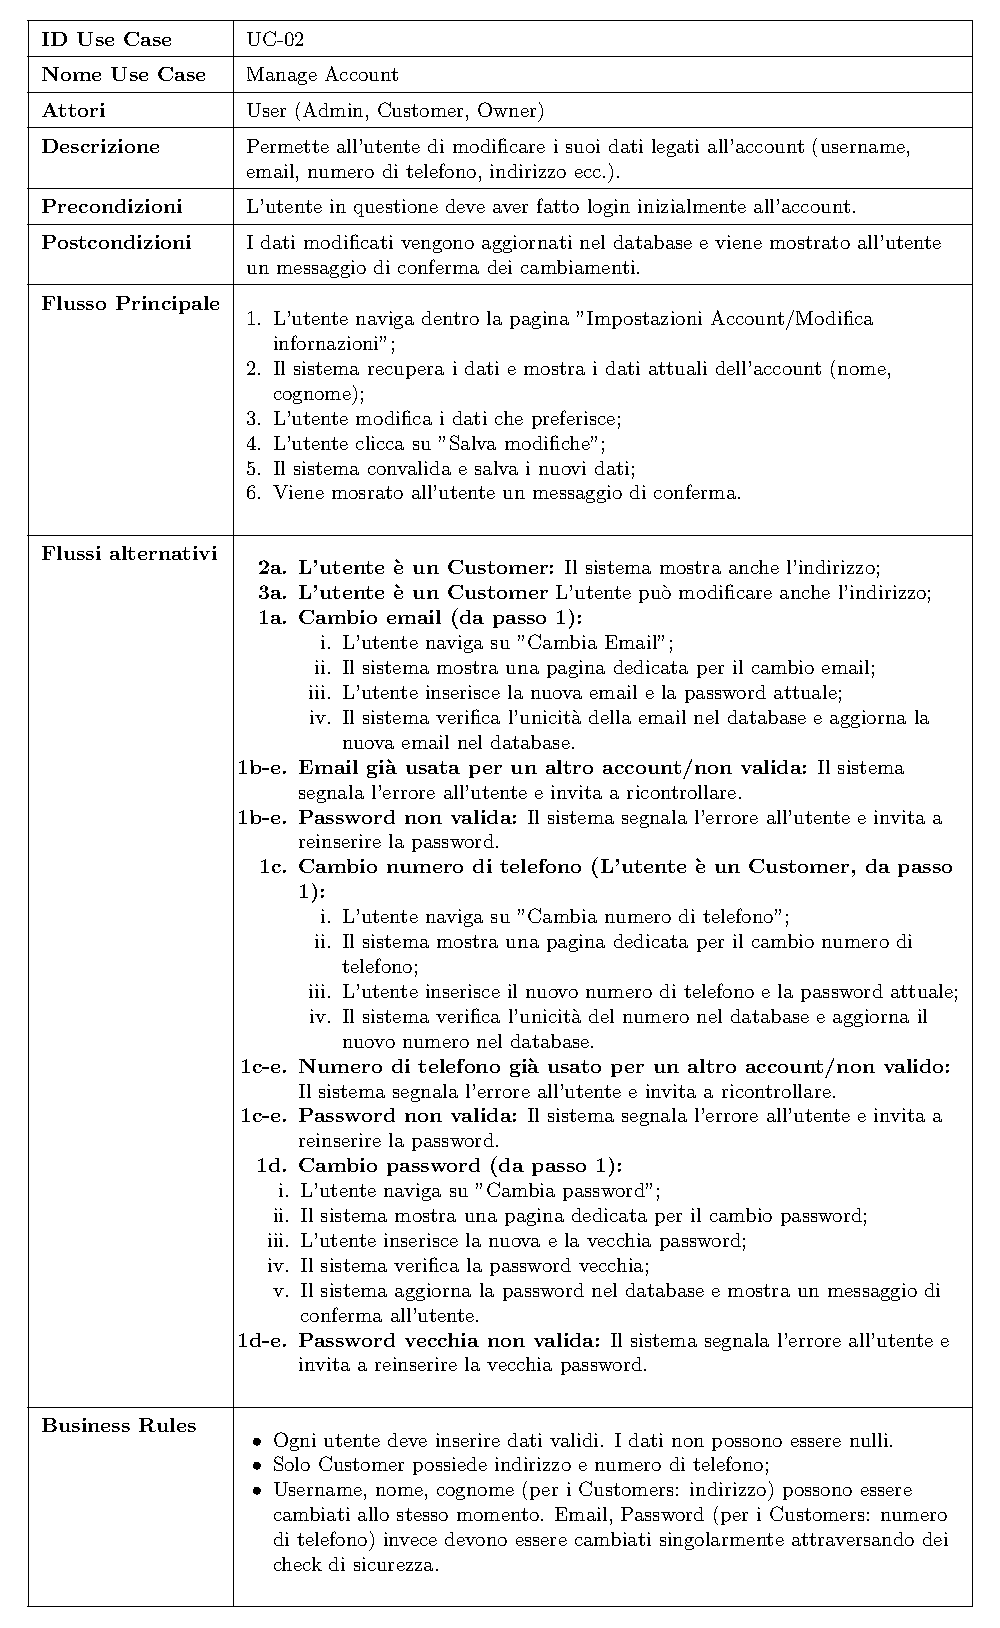
\includegraphics[width=0.85\linewidth]{UC02/UC02.pdf}
    }
    \caption{UC: Manage Account}
    \label{fig:UC02}
\end{figure}

\subsubsection{Create Booking}

\begin{figure}[H]
    \centering
    \makebox[\textwidth][c]{
        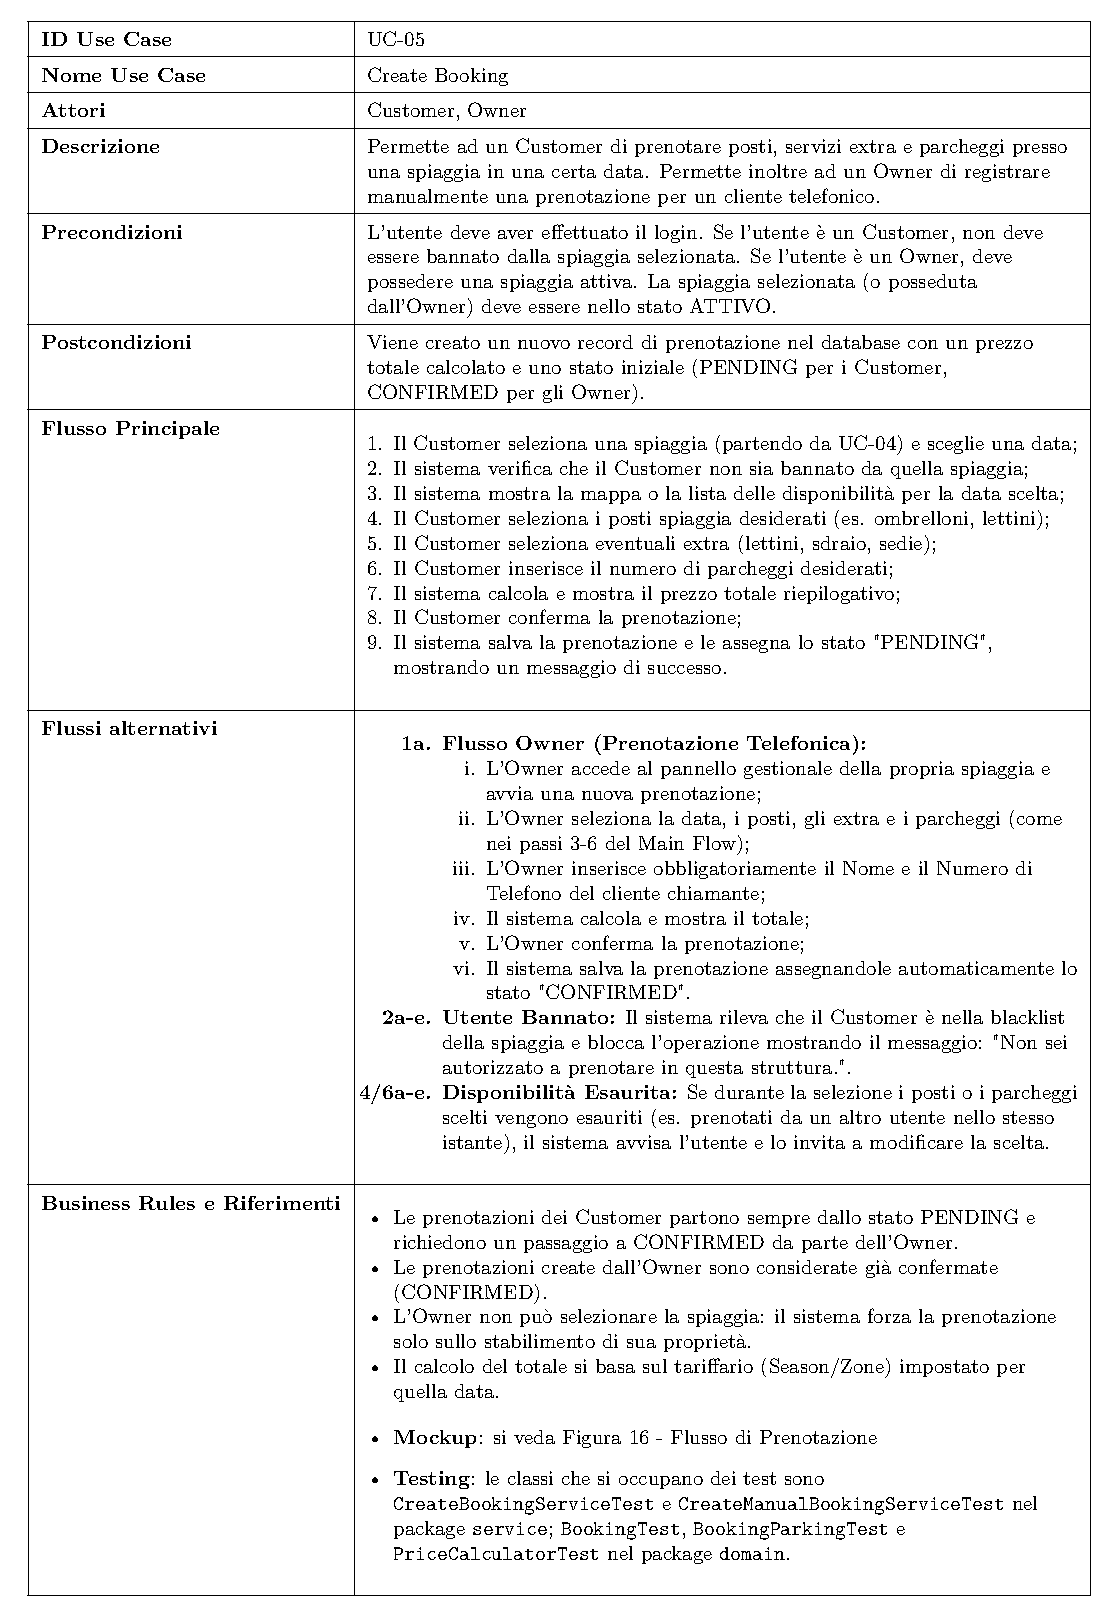
\includegraphics[width=0.85\textwidth]{UC05/UC05.pdf}
    }
    \caption{UC: Create Booking}
    \label{fig:UC05}
\end{figure}

\subsubsection{Manage Reviews}

\begin{figure}[H]
    \centering
    \makebox[\textwidth][c]{
        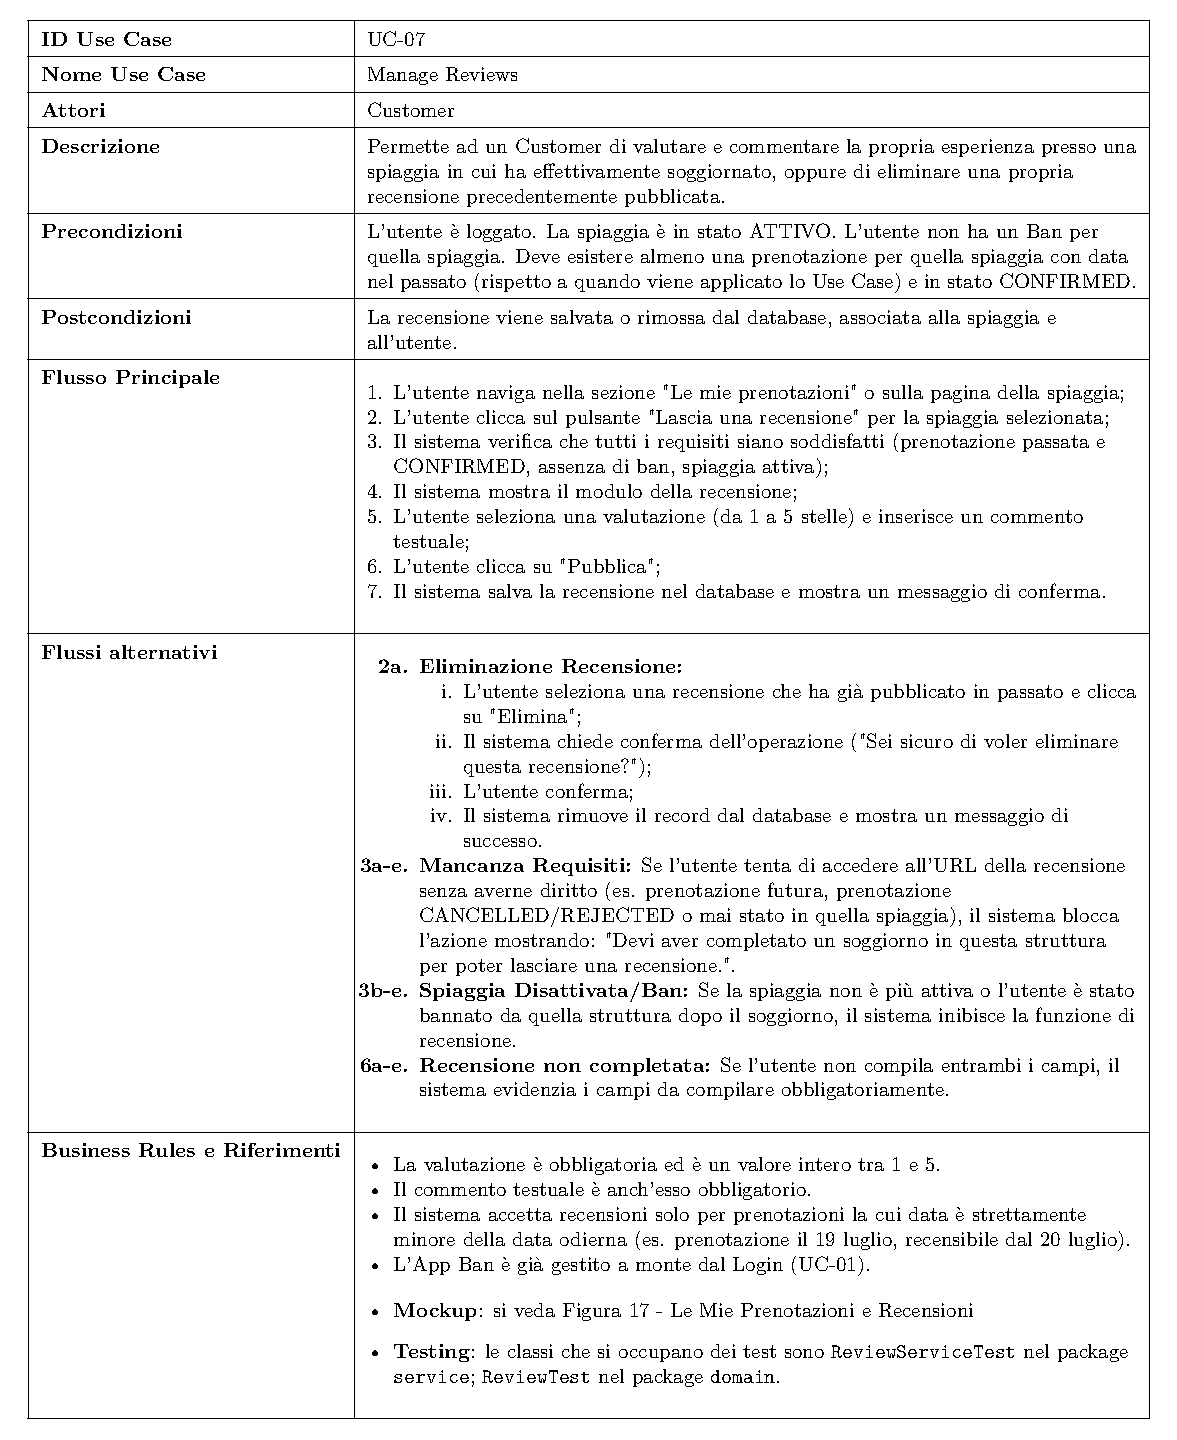
\includegraphics[width=0.85\textwidth]{UC07/UC07.pdf}
    }
    \caption{UC: Manage Reviews}
    \label{fig:UC07}
\end{figure}

\subsubsection{Create Beach}

\begin{figure}[H]
    \centering
    \makebox[\textwidth][c]{
        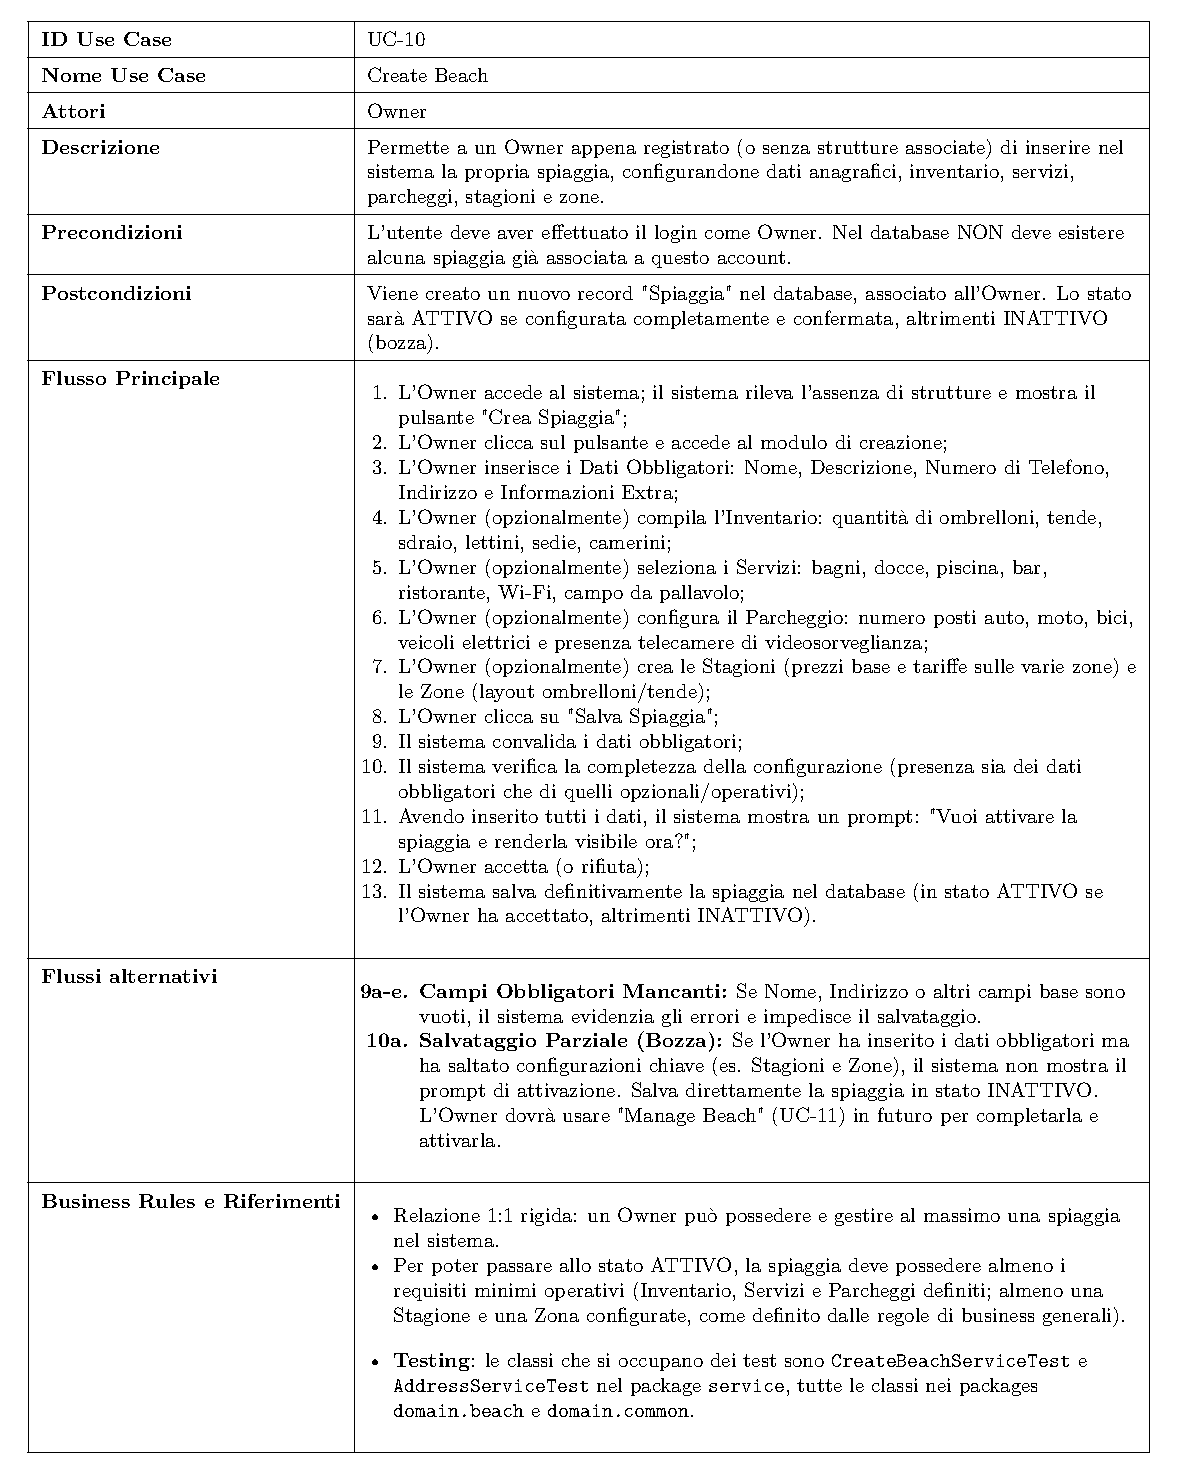
\includegraphics[width=0.85\textwidth]{UC10/UC10.pdf}
    }
    \caption{UC: Create Beach}
    \label{fig:UC10}
\end{figure}

\subsubsection{Manage Beach}

\begin{figure}[H]
    \centering
    \makebox[\textwidth][c]{
        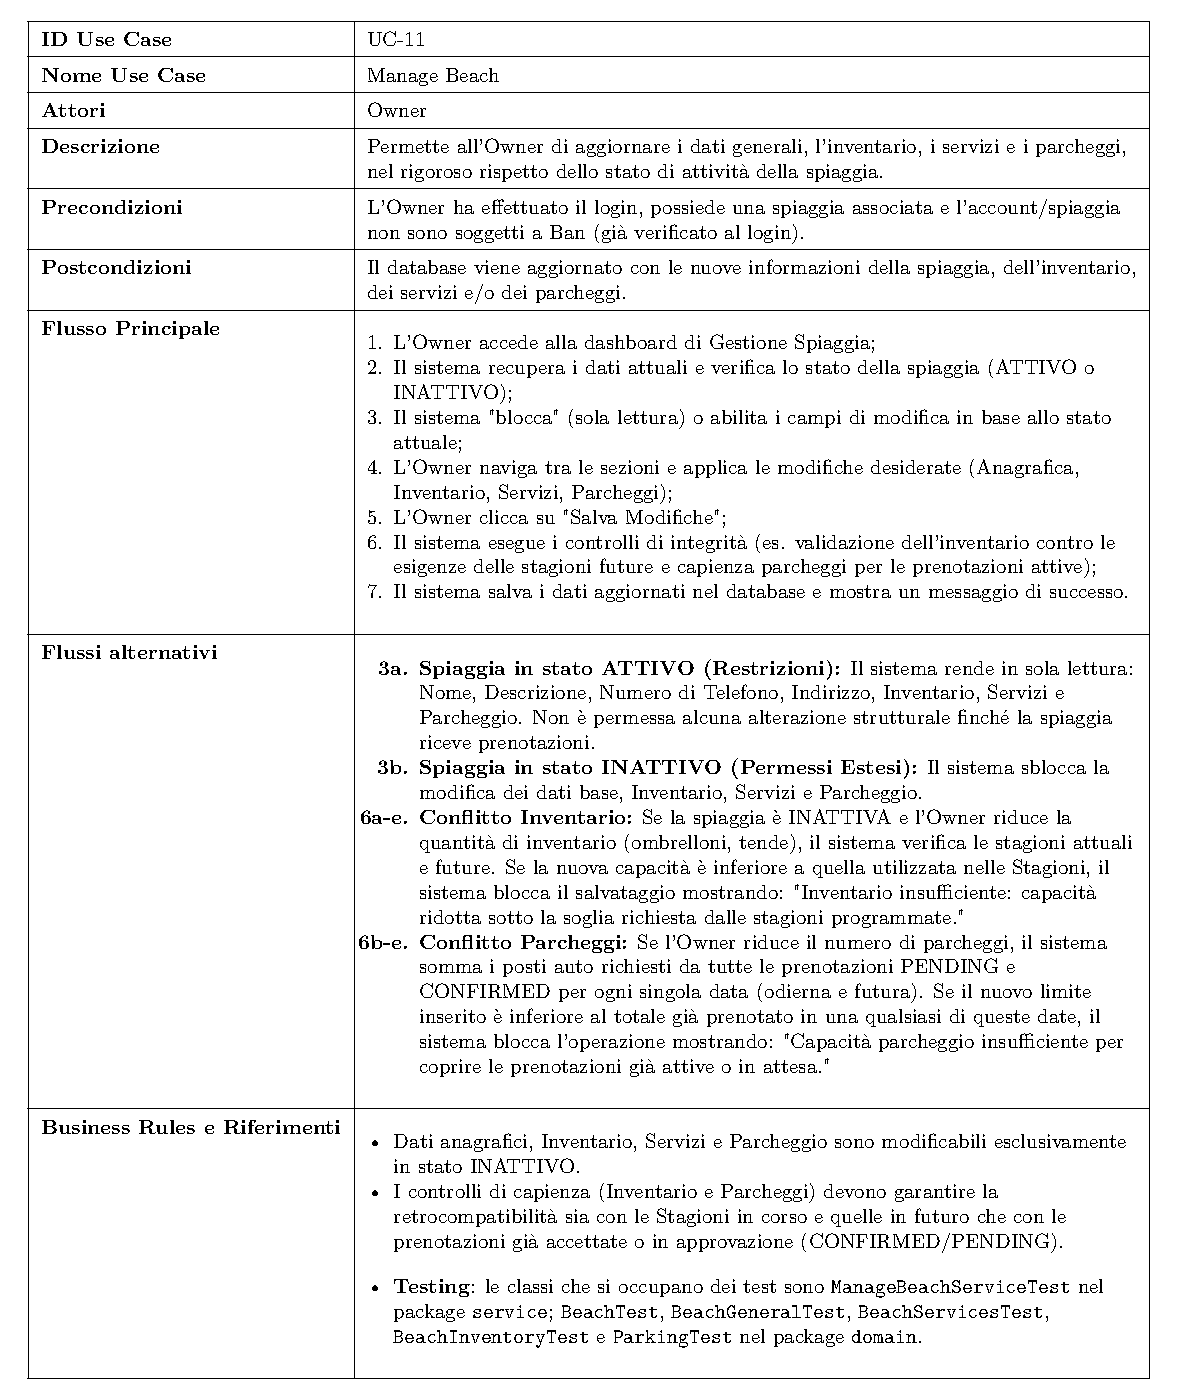
\includegraphics[width=0.85\textwidth]{UC11/UC11.pdf}
    }
    \caption{UC: Manage Beach}
    \label{fig:UC11}
\end{figure}

\newpage

\section{Progettazione}
\label{cap:Progettazione}

\subsection{Pattern Architetturali e Progettuali}
\label{cap:Pattern}

Per lo sviluppo di SunSpot sono stati adottati diversi pattern volti a garantire un'architettura robusta, testabile e facilmente manutenibile, separando nettamente le responsabilità tra logica di business e dettagli implementativi.

\subsubsection{Architettura Esagonale (Ports \& Adapters)}
Il progetto SunSpot adotta i principi dell'Architettura Esagonale per garantire una separazione  delle responsabilità e un totale isolamento della logica di business dalle tecnologie esterne. L'architettura prevede un nucleo centrale (\textbf{Core}), composto dai package \texttt{domain} e \texttt{application}, e un perimetro esterno, composto dagli \textbf{Adapters} nel package \texttt{infrastructure.persistence.jdbc}.

Lo strato di \textbf{Application} funge da ponte tra il mondo esterno e il dominio ed è suddiviso in due componenti fondamentali:
\begin{itemize}
    \item \textbf{Ports (Interfacce)}: rappresentano i contratti di comunicazione dell'esagono. Si distinguono in:
    \begin{itemize}
        \item \textbf{Port-In (Driving Ports)}: definiscono i casi d'uso e le azioni che gli attori esterni possono richiedere al sistema (es. \autoref{lst:UseCase}).
        \item \textbf{Port-Out (Driven Ports)}: definiscono i requisiti infrastrutturali necessari al (\textbf{Core}) per funzionare (es. \autoref{lst:Repository}).
    \end{itemize}
    
    \item \textbf{Services (Orchestratori)}: rappresentano le implementazioni concrete delle Port-In. Il loro ruolo è quello di \textbf{orchestratori dei casi d'uso}: un Service riceve un comando, recupera i dati necessari tramite le Port-Out, delega la logica decisionale e di validazione alle entità del \texttt{domain} e infine persiste i cambiamenti tramite le Port-Out. Il Service non contiene logica di business, ma si occupa esclusivamente di coordinare il flusso operativo e gestire l'integrità delle transazioni.
\end{itemize}

Grazie a questa struttura, il sistema gode di una notevole resilienza; l'utilizzo delle interfacce assicura che il \textbf{disaccoppiamento} sia totale. Se in futuro fosse necessario migrare verso un diverso sistema di persistenza o un servizio cloud, sarebbe sufficiente sviluppare un nuovo Adapter senza dover modificare il codice nel Core applicativo.

\begin{lstlisting}[caption={Esempio Port-In (Contratto dei casi d'uso)}, label={lst:UseCase}]
public interface BookingUseCase {
    void confirmBooking(Integer id);
    void cancelBooking(Integer id);
    
    // ... altri metodi omessi ...
    List<Booking> getCustomerBookings(Integer customerId);
}
\end{lstlisting}

\begin{lstlisting}[caption={Esempio Port-Out (Requisiti verso il Database)}, label={lst:Repository}]
public interface BookingRepository {
    Integer save(Booking booking, TransactionContext context);
    void update(Booking booking, TransactionContext context);

    Optional<Booking> findById(Integer id, TransactionContext context);
    List<Integer> findOccupiedSpots(Integer beachId, LocalDate date, TransactionContext context);
}
\end{lstlisting}

\begin{lstlisting}[caption={Esempio Service (Orchestrazione e Transazionalità)}, label={lst:Service}]
public class BookingService implements BookingUseCase {
    // ... attributi e costruttore (Dependency Injection) ...
    
    @Override
    public void confirmBooking(Integer id) {
        transactionManager.executeInTransaction(context -> {
            Booking booking = getBookingOrThrow(id, context);

            // Delegazione della logica di validazione al Dominio
            booking.confirmBooking();

            // Persistenza dello stato modificato
            bookingRepository.update(booking, context);
        });
    }
 }   
\end{lstlisting}

\subsubsection{DDD-lite (Domain-Driven Design)}
A integrazione dell'architettura esagonale, è stato adottato l'approccio \textbf{DDD-lite}. Mentre l'esagonale definisce i confini, il \textbf{DDD} stabilisce che il nucleo del progetto deve riflettere il linguaggio e le regole della realtà modellata. 

Il cuore di questo approccio è il \textbf{Rich Domain Model}; a differenza di un modello anemico (fatto di soli getter e setter), nel nostro dominio le entità hanno il compito di assicurarsi l'integrità dei dati sia in fase di modifica che di instanziamento. Ad esempio: la classe \texttt{Beach} presenta metodi interni dedicati a controllare la presenza di tutti i dati obbligatori e il rispetto dei vincoli di business prima che l'oggetto possa essere effettivamente creato o modificato  (es. \autoref{lst:Entities}).

In questa architettura abbiamo distinto:
\begin{itemize}
    \item \textbf{Entities}: oggetti con un'identità univoca che persiste nel tempo (es. \autoref{lst:Entities}).
    \item \textbf{Value Objects}: oggetti definiti dai propri attributi e immutabili, implementati tramite i \textbf{Java Records} (es. \autoref{lst:ValueObjects}).
\end{itemize}

\newpage
 \begin{lstlisting}[caption={Esempio Entity (Integrità dello stato e logica di business)}, label={lst:Entities}]
public class Beach {
    private final Integer id; // Identita univoca
    private BeachInventory beachInventory; // Value Object composito
    private boolean active;
    private boolean closed;

    // ... costruttore omesso ...

    // Metodo di dominio con validazione interna
    public void setActive(boolean active) {
        if (active) {
            validateActivationRequirements();
        }
        this.active = active;
    }

    private void validateActivationRequirements() {
        if (beachInventory == null) throw new IllegalStateException("Missing inventory");
        // ... altri controlli di business ...
    }
}
\end{lstlisting}
 
Un aspetto centrale nella progettazione è la gestione del ciclo di vita dei \textbf{Value Objects}, improntata alla massima protezione dello stato tramite due principi cardine:

\begin{itemize}
    \item \textbf{Ricostruzione del Modello}: Le entità non vengono semplicemente "lette" dal database, ma \textit{ricostituite}. Lo strato di persistenza fornisce i dati affinché il Core possa istanziare nuovamente l'entità, garantendo che i vincoli vengano verificati nel momento stesso della creazione in memoria.
    \item \textbf{Metodi Wither e Immutabilità}: Invece di alterare lo stato di un'istanza esistente tramite \textit{setter}, le modifiche generano una \textbf{nuova istanza} dell'oggetto (\autoref{lst:ValueObjects}). Questo garantisce l'immutabilità durante il ciclo di vita in memoria, facilitando il debugging e assicurando la consistenza tra gli strati applicativi.
\end{itemize}

\begin{lstlisting}[caption={Value Object: Integrità alla creazione e pattern Wither}, label={lst:ValueObjects}]
public record BeachInventory(int countExtraSdraio, int countCamerini) {
    
    // Costruttore compatto per validare le regole di business
    public BeachInventory {
        if (countExtraSdraio < 0 || countCamerini < 0) {
            throw new IllegalArgumentException("ERROR: counts cannot be negative");
        }
    }

    // Metodo Wither: crea una nuova istanza immutabile con un dato aggiornato
    public BeachInventory withCountCamerini(int countCamerini) {
        return new BeachInventory(this.countExtraSdraio, countCamerini);
    }
}
\end{lstlisting}

\subsubsection{Builder Pattern}
Il pattern Builder è stato utilizzato per gestire l'instanziamento di classi caratterizzate da un elevato numero di parametri e attributi opzionali, evitando costruttori eccessivamente complessi e verbosi. Tramite una classe interna statica la costruzione dell'oggetto avviene in modo guidato e leggibile (es. \autoref{lst:Builder}).

Il pattern è stato applicato a classi come \texttt{Address}, \texttt{Spot}, \texttt{Zone} e ai \textit{Value-Objects} associati a \texttt{Booking} e \texttt{Beach}. In particolare nel caso della spiaggia, vista la densità di informazioni richieste, abbiamo suddiviso gli attributi in diversi \textit{Value-Objects}, ciascuno dei quali viene istanziato tramite il proprio builder. Questo
 permette di gestire con estrema facilità la configurazione di parametri non obbligatori, mantenendo il codice pulito e uniforme in tutto il progetto.
 
 \begin{lstlisting}[caption={Implementazione del pattern Builder su un Value Object}, label={lst:Builder}]
public static class Builder {
    private int countExtraSdraio = 0;
    private int countCamerini = 0;

    public Builder countExtraSdraio(int val) {
        this.countExtraSdraio = val;
        return this; // Permette il method chaining
    }

    public BeachInventory build() {
        // La validazione avverra automaticamente nel costruttore del Record
        return new BeachInventory(countExtraSdraio, countCamerini);
    }
}
\end{lstlisting}


\newpage
\subsection{Struttura del codice}

La struttura della directory del progetto è stata organizzata in base alla separazione dei package di Java e seguendo i principi dell'architettura software a livelli, descritta precedentemente.

\begin{verbatim}
|-- .idea
|-- .mvn
|-- db-init
|-- src
|   |-- main
|   |   |-- java
|   |   |   |-- com.example.s_balneare
|   |   |       |-- application
|   |   |       |   |-- port
|   |   |       |   |    |--in
|   |   |       |   |    |-out
|   |   |       |   |-- service
|   |   |       |-- domain
|   |   |       |-- infrastructure.persistence.jdbc
|   |   |       |-- Main.java
|   |   |       |-- module-info.java
|   |   |-- resources
|   |-- test
|       |-- java
|           |-- com.example.s_balneare
|               |-- application
|               |     |--service
|               |-- domain
|               |-- AllTestsSuite.java
|               |-- ApplicationTestSuite.java
|               |-- DomainTestSuite.java
|-- target
|-- .gitignore
|-- docker-compose.yml
\end{verbatim}



La directory dei test rispecchia la struttura principale per mantenere gli Unit Test organizzati (con package paralleli come \texttt{application} e \texttt{domain} e le relative Test Suite). L'adozione di queste pratiche garantisce un progetto chiaro, strutturato e facilmente manutenibile, evitando al contempo problemi legati alla visibilità dei package.

Ogni package interagisce con gli altri per svolgere compiti specifici, mantenendo una netta separazione tra il dominio applicativo (\texttt{domain}) , i casi d'uso (\texttt{application}) e la gestione dei dati e interazioni con il database (\texttt{infrastructure.persistence.jdbc}). Tale approccio strutturato assicura che ogni componente del sistema abbia una responsabilità ben definita, rendendo il codice più facile da navigare, comprendere ed estendere. Inoltre facilita la collaborazione tra i membri del team, poiché ogni package può essere sviluppato e testato in modo indipendente.

\newpage

\subsection{Domain}
Il livello di \textbf{Domain} rappresenta il nucleo fondante dell'applicazione, in cui risiedono le regole di business e la modellazione dello stato. In conformità ai principi del pattern \textbf{DDD-lite}, le classi non sono meri contenitori di dati, ma garantiscono autonomamente l'integrità del sistema.
La struttura gerarchica e relazionale delle entità è sintetizzata nel diagramma UML riportato in \autoref{fig:domain_UML}.
% HO AGGIUNTO QUESTO PARAGRAFINO. SE NON TI PIACE TOGLILO!!!
Per il diagramma completo, con metodi e attributi di ciascuna classe, si veda \href{run:img/domainUML.pdf}{il seguente PDF}.

Dal punto di vista architetturale, la relazione tra \textbf{Entities} e \textbf{Value Objects} si concretizza tramite il principio della \textit{composizione}: le Entità incapsulano i Value Objects come propri attributi, delegando a questi ultimi la gestione di raggruppamenti logici e immutabili di dati (ad esempio, le informazioni generali o l'inventario di una spiaggia).

Per quanto riguarda la modellazione degli attori principali del sistema (\textit{Customer}, \textit{Owner} e \textit{Admin}), si è optato per un approccio basato sull'\textbf{ereditarietà}. Tutti i ruoli estendono una classe base \texttt{User}, permettendo di centralizzare le funzionalità e le anagrafiche comuni, sfruttando il polimorfismo al fine di semplificare l'estensibilità del codice.
\begin{figure}[H] 
    \centering
    \begin{adjustbox}{max width=1.15\textwidth, max totalheight=0.9\textheight, center}
        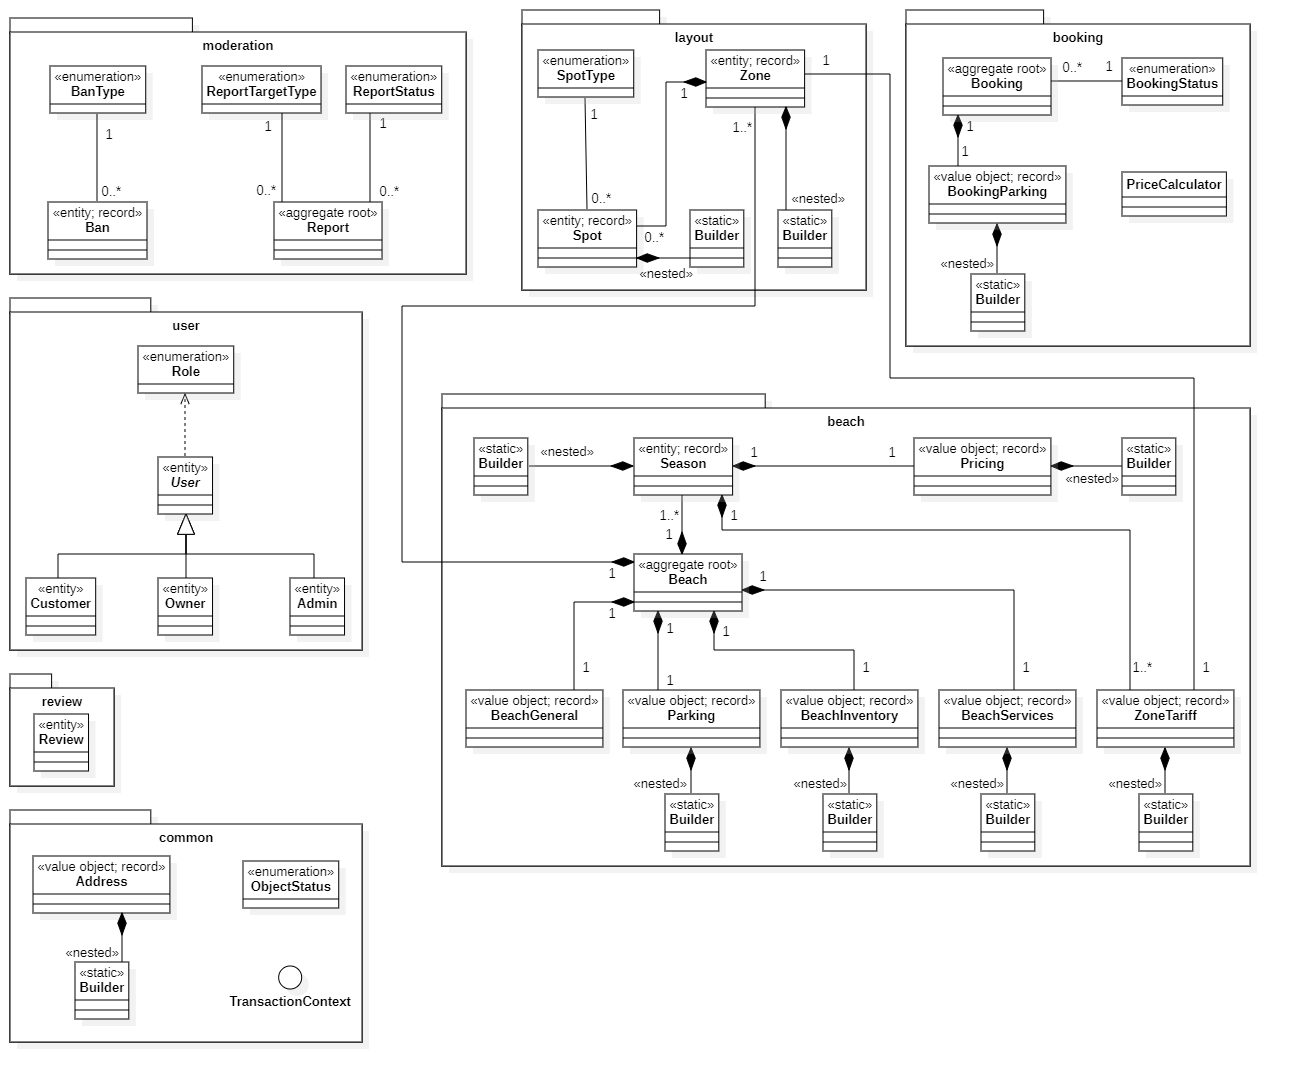
\includegraphics{img/UML domain(solo classi).png}
    \end{adjustbox}
    \caption{Domain UML}
    \label{fig:domain_UML}
\end{figure}

\subsection{Application}
Il livello applicativo ha  il compito di interconnettere  il cuore del  progetto con  il mondo esterno tramite gli strumenti precedentemente elencati.
\subsubsection{Port-out}
Nel  progetto, le \textbf{Port-Out} sono interfacce Java che definiscono i requisiti di persistenza e le interazioni esterne in modo astratto e universale. Questo approccio permette alla logica di business di invocare i metodi necessari senza dipendere dalla reale implementazione tecnologica sottostante. L'implementazione di queste interfacce è affidata al package \texttt{infrastructure.persistence.jdbc}, il quale ha il compito di tradurre le azioni dettate dal dominio in istruzioni JDBC per il database MySQL. Tale package include inoltre diversi \textbf{Record} (evidenziati in rosso nella \autoref{fig:PortOut}), utilizzati come strutture dati (DTO) per veicolare le informazioni estratte dal database affinché siano adatte per essere elaborate dai metodi del core applicativo.
\begin{figure}[H]
	\centering

	% --- RIGA 1: ROOT E BEACH ---
	\begin{minipage}[t]{0.48\textwidth}
		\begin{lstlisting}[frame=none, basicstyle=\ttfamily\footnotesize]
			out/
			|-- beach/
			|-- booking/
			|-- common/
			|-- moderation/
			|-- review/
			|-- user/
			|-- TransactionManager.java
		\end{lstlisting}
    \end{minipage}\hfill
    \begin{minipage}[t]{0.48\textwidth}
		\begin{lstlisting}[frame=none, basicstyle=\ttfamily\footnotesize]
		beach/
		|-- BeachCatalogQuery.java
		|-- BeachRepository.java
		|-- (*@\color{red}BeachReviewDto.java@*)
		|-- BeachReviewsQuery.java
		|-- (*@\color{red}BeachSummary.java@*)
		\end{lstlisting}
    \end{minipage}\vspace{0.8cm}

    % --- RIGA 2: BOOKING E USER ---
    \begin{minipage}[t]{0.48\textwidth}
		\begin{lstlisting}[frame=none, basicstyle=\ttfamily\footnotesize]
		booking/
		|-- AvailabilityQuery.java
		|-- (*@\color{red}BookedInventory.java@*)
		|-- (*@\color{red}BookedParkingSpaces.java@*)
		|-- BookingRepository.java
		\end{lstlisting}
    \end{minipage}\hfill
    \begin{minipage}[t]{0.48\textwidth}
		\begin{lstlisting}[frame=none, basicstyle=\ttfamily\footnotesize]
		user/
		|-- AdminRepository.java
		|-- AuthenticationUseCase.java
		|-- CustomerRepository.java
		|-- (*@\color{red}LoginResult.java@*)
		|-- OwnerRepository.java
		|-- UserRepository.java
		\end{lstlisting}
    \end{minipage}\vspace{0.8cm}

    % --- RIGA 3: MODERATION E ALTRI ---
    \begin{minipage}[t]{0.48\textwidth}
		\begin{lstlisting}[frame=none, basicstyle=\ttfamily\footnotesize]
		moderation/
		|-- BanRepository.java
		|-- ReportRepository.java
		\end{lstlisting}
    \end{minipage}\hfill
    \begin{minipage}[t]{0.48\textwidth}
		\begin{lstlisting}[frame=none, basicstyle=\ttfamily\footnotesize]
		common/
		|-- AddressRepository.java
		
		review/
		|-- ReviewRepository.java
		\end{lstlisting}
    \end{minipage}
    \caption{Struttura delle Port-Out}
    \label{fig:PortOut}
\end{figure}
Il \textbf{TransactionManager} è l'interfaccia dedicata alla gestione del ciclo di vita delle transazioni, assicurando che il flusso di operazioni sul database rispetti le proprietà \textbf{ACID} (Atomicità, Consistenza, Isolamento e Durata). Il componente implementa il pattern \textbf{Unit of Work} attraverso l'uso di un oggetto \textbf{TransactionContext}. 

Questo contesto, definito tramite un'interfaccia marker, viene condiviso esplicitamente come parametro a ogni metodo delle repository coinvolto nel caso d'uso (es. \texttt{beachRepository.update(beach, context)}). Tale meccanismo garantisce che tutte le operazioni effettuate all'interno di un blocco transazionale siano atomiche: in caso di successo di ogni passaggio, il manager esegue il \textit{commit} dei dati sul database; qualora venisse sollevata un'eccezione (es. un errore di sicurezza o validazione), il manager interviene eseguendo un \textit{rollback} automatico per preservare l'integrità e la consistenza dello stato persistente.
\subsubsection{Port-in}
Le \textbf{Port-In} (o \textit{Driving Ports}) rappresentano i punti di ingresso all'esagono applicativo. Esse definiscono formalmente i casi d'uso e le azioni che gli attori esterni (come l'interfaccia utente o sistemi di test) possono richiedere al sistema. 

In questa architettura, le Port-In sono strutturate attraverso due componenti principali:
\begin{itemize}
    \item \textbf{UseCase (Interfacce Java)}: definiscono i contratti delle operazioni di business. Esse dettano quali informazioni sono necessarie per eseguire un'azione e garantiscono che il mondo esterno interagisca con il core solo attraverso canali controllati,
    \item \textbf{Command e Request (Input Models)}: rappresentati spesso come \textit{Java Record} (evidenziati in rosso nella \autoref{fig:PortIn}), questi oggetti fungono da contenitori di dati immutabili. Il loro compito è veicolare i parametri necessari per l'esecuzione del caso d'uso, permettendo una validazione sintattica preliminare prima che la richiesta raggiunga la logica di business.
\end{itemize}

L'implementazione concreta di queste interfacce è affidata al livello \textbf{Service}. I servizi orchestrano il flusso chiamando correttamente i metodi definiti dalle Port-Out e delegando le regole decisionali alle entità del dominio, assicurando così che ogni richiesta venga elaborata in modo coerente e sicuro.

\begin{figure}[H]
    \centering

    % --- RIGA 1: ROOT E BEACH ---
    \begin{minipage}[t]{0.48\textwidth}
		\begin{lstlisting}[frame=none, basicstyle=\ttfamily\footnotesize]
		in/
		|-- beach/
		|-- booking/
		|-- common/
		|-- moderation/
		|-- review/
		|-- user/
		\end{lstlisting}
    \end{minipage}\hfill
    \begin{minipage}[t]{0.48\textwidth}
		\begin{lstlisting}[frame=none, basicstyle=\ttfamily\footnotesize]
		beach/
		|-- BrowseBeachUseCase.java
		|-- CloseBeachUseCase.java
		|-- (*@\color{red}CreateBeachCommand.java@*)
		|-- CreateBeachUseCase.java
		|-- ManageBeachUseCase.java
		\end{lstlisting}
    \end{minipage}\vspace{0.8cm}

    % --- RIGA 2: BOOKING E USER ---
    \begin{minipage}[t]{0.48\textwidth}
		\begin{lstlisting}[frame=none, basicstyle=\ttfamily\footnotesize]
		booking/
		|-- BookingUseCase.java
		|-- (*@\color{red}CreateBookingCommand.java@*)
		|-- CreateBookingUseCase.java
		|-- (*@\color{red}CreateManualBookingCommand.java@*)
		|-- CreateManualBookingUseCase.java
		\end{lstlisting}
    \end{minipage}\hfill
    \begin{minipage}[t]{0.48\textwidth}
		\begin{lstlisting}[frame=none, basicstyle=\ttfamily\footnotesize]
		user/
		|-- (*@\color{red}CreateAdminRequest.java@*)
		|-- (*@\color{red}CreateCustomerRequest.java@*)
		|-- (*@\color{red}CreateOwnerRequest.java@*)
		|-- (*@\color{red}CreateUserRequest.java@*)
		|-- UserRegistrationUseCase.java
		\end{lstlisting}
    \end{minipage}\vspace{0.8cm}

    % --- RIGA 3: MODERATION E REVIEW ---
    \begin{minipage}[t]{0.48\textwidth}
		\begin{lstlisting}[frame=none, basicstyle=\ttfamily\footnotesize]
		moderation/
		|-- BanUseCase.java
		|-- (*@\color{red}CreateBanCommand.java@*)
		|-- (*@\color{red}CreateReportCommand.java@*)
		|-- CreateReportUseCase.java
		|-- ManageReportUseCase.java
		\end{lstlisting}
    \end{minipage}\hfill
    \begin{minipage}[t]{0.48\textwidth}
		\begin{lstlisting}[frame=none, basicstyle=\ttfamily\footnotesize]
		review/
		|-- (*@\color{red}CreateReviewCommand.java@*)
		|-- ReviewUseCase.java
		|-- ViewBeachReviewsUseCase.java
		
		common/
		|-- AddressUseCase.java
		\end{lstlisting}
    \end{minipage}
    \caption{Struttura delle Port-In}
    \label{fig:PortIn}
\end{figure}

\newpage

\section{Database}
Per la gestione della persistenza dei dati è stato utilizzato il DBMS \textbf{MySQL}, configurato all'interno di un ambiente di containerizzazione \textbf{Docker}. L'interazione tra l'applicazione Java e il database avviene tramite l'interfaccia \textbf{JDBC}, utilizzando il driver ufficiale \textbf{MySQL Connector/J}.

L'integrità del dato è assicurata a livello nativo attraverso una rigorosa definizione di vincoli (Foreign Key, Unique e Check) implementati nello script di creazione. Tale approccio permette di delegare al database la validazione delle informazioni critiche, mentre le verifiche legate alla \textbf{logica di business} sono gestite programmaticamente all'interno del codice Java dell'applicazione.

\subsection{Modello ER}
Il modello Entity-Relationship (\autoref{fig:modelloER}) omette la relazione diretta tra \textit{Beaches} e \textit{Bookings} per evitare ridondanze concettuali, essendo il legame già mediato dalle entità \textit{Zones} e \textit{Spots}. In fase di implementazione del database fisico, tuttavia, tale relazione è stata introdotta per ottimizzare le performance delle query di ricerca, riducendo la complessità delle operazioni di join.

\begin{figure}[H] 
    \centering
     \makebox[\textwidth][c]{   
     \includegraphics[width=1.15\textwidth]{ModelloER.pdf} 
     }
    \caption{Modello Entity Relationship (Schema Concettuale)}
    \label{fig:modelloER}
\end{figure}

\newpage

\subsection{Dizionario dei dati}
Il dizionario (\autoref{fig:diz_entita} e \autoref{fig:diz_relazioni}) presenta per \textit{Spots} e \textit{Bookings} attributi identificativi esterni derivanti dalle relazioni con altre entità. Per semplificare le interrogazioni e la realizzazione del database si è optato per l'utilizzo di una chiave primaria artificiale (\textit{id}), preservando la valenza identificativa di questi attributi tramite vincoli \texttt{UNIQUE} e \texttt{NOT NULL}, come dettagliato nella tabella dei vincoli (\autoref{fig:tab_vincoli}).

\begin{figure}[H]
    \centering
    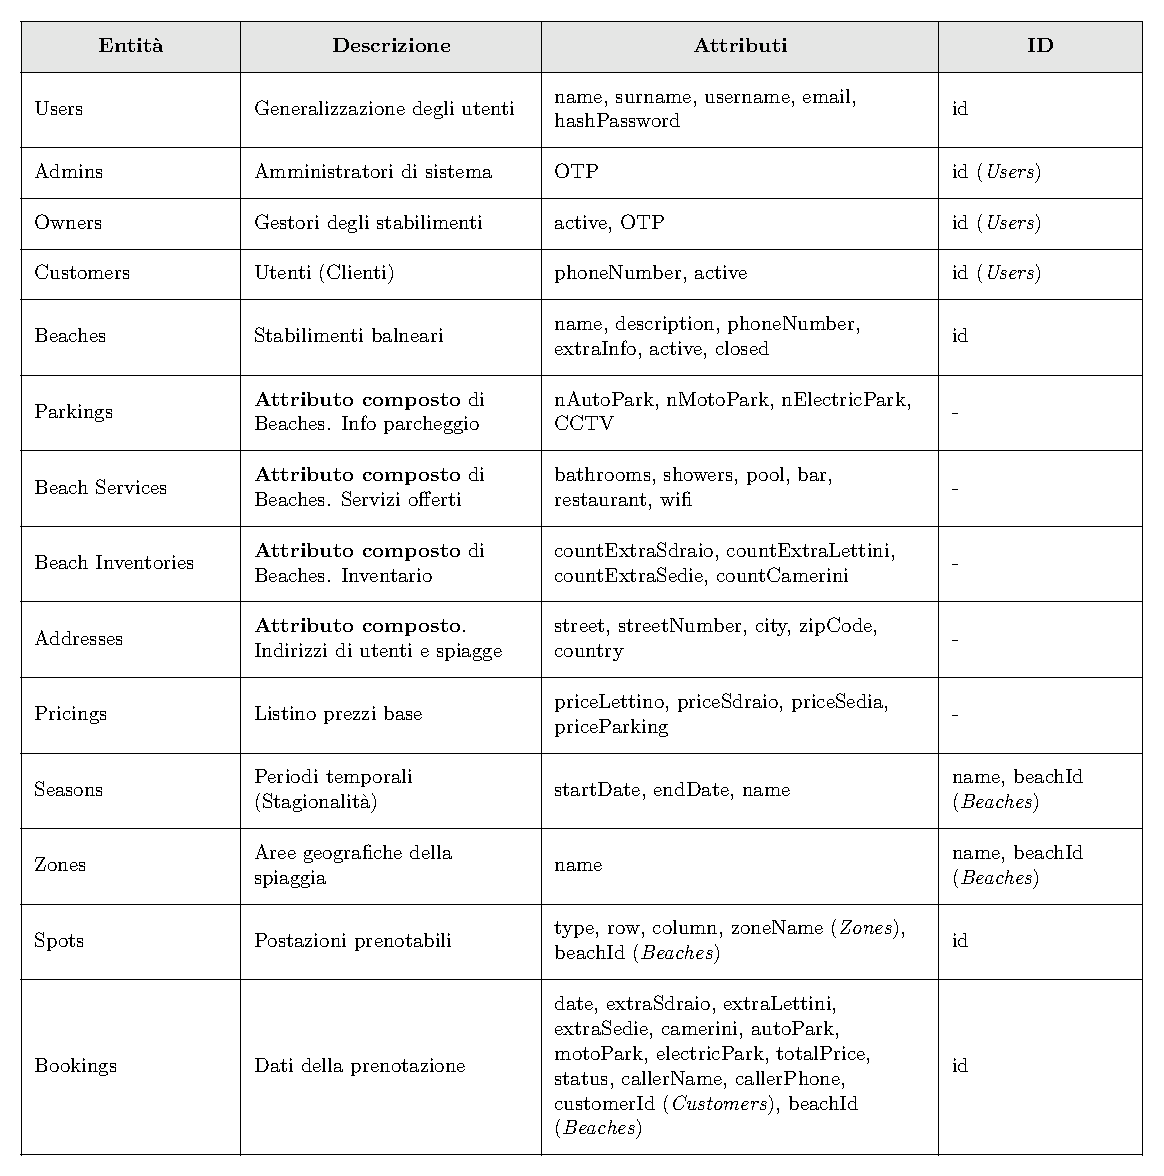
\includegraphics[width=1\textwidth]{DataBase/Dizionario/Entità}
    \caption{Dizionario delle Entità}
    \label{fig:diz_entita}
\end{figure}

\begin{figure}[H]
    \centering
    \includegraphics[width=1\textwidth]{DataBase/Dizionario/relazioni}
    \caption{Dizionario delle Relazioni}
    \label{fig:diz_relazioni}
\end{figure}

\newpage

\subsection{Tabelle delle Regole}
Di seguito vengono riportati i vincoli di integrità e le regole di derivazione che governano la logica della persistenza dei dati.
In merito alla regola RD1 (\autoref{fig:tab_derivazioni}), si è scelta la persistenza dell'attributo \textit{totalPrice} nel database al fine di ridurre il carico computazionale di consultazione.

\begin{figure}[H]
	\centering
	
	\begin{subfigure}{\textwidth}
		\centering
		\includegraphics[width=0.85\textwidth]{DataBase/Tabelle/vincoli}
		\caption{Tabella dei vincoli di integrità (RV)}
	\end{subfigure}
	
	\vspace{0.5cm}
	
	\begin{subfigure}{\textwidth}
		\centering
		\includegraphics[width=0.9\textwidth]{DataBase/Tabelle/derivazioni}
		\caption{Tabella delle regole di derivazione (RD)}
		\label{fig:tab_derivazioni}
	\end{subfigure}
	
	\caption{Tabelle delle Regole}
	\label{fig:tabelle}
\end{figure}

\newpage

\section{Mockup}

In questa sezione vengono presentati i mockup dell'interfaccia grafica, realizzati con lo scopo di dimostrare visivamente come i requisiti e le rigide regole di business (definite nel Domain-Driven Design) si traducano nell'esperienza utente finale. 

Per ottimizzare i tempi di prototipazione e ottenere un design moderno e responsivo, sono stati impiegati due strumenti di generazione UI basati sull'Intelligenza Artificiale:
\begin{itemize}
	\item \textbf{v0.dev (Vercel):} utilizzato per generare i primi 4 mockup, focalizzati sull'esperienza Mobile (B2C) dedicata ai \textit{Customer}.
	\item \textbf{bolt.new (StackBlitz):} utilizzato per generare gli ultimi 4 mockup, focalizzati sulle Dashboard Desktop (B2B) destinate alla gestione avanzata da parte di \textit{Owner} e \textit{Admin}.
\end{itemize}

\begin{figure}[H]
	\centering
	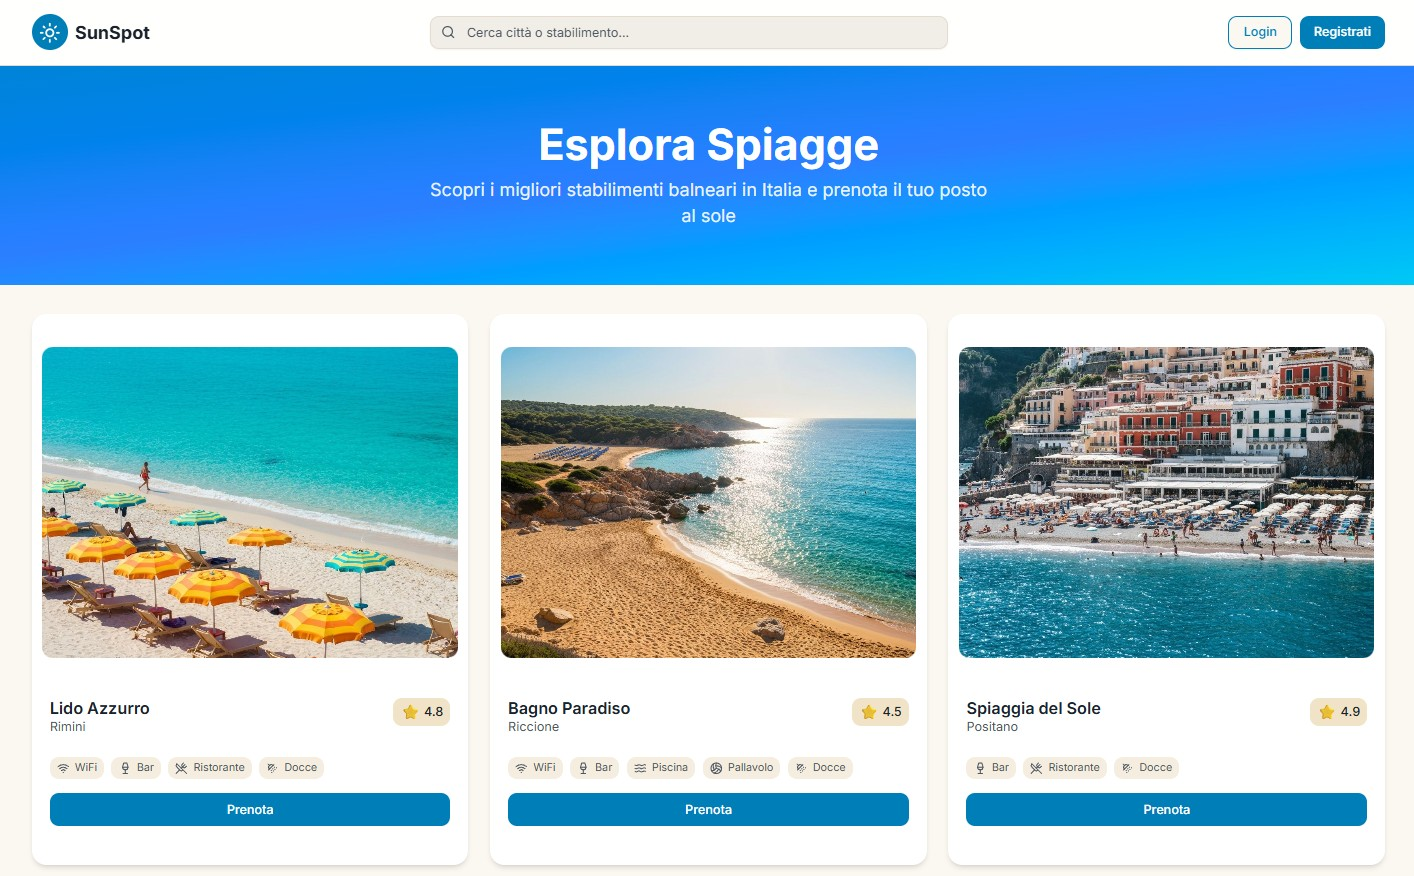
\includegraphics[width=0.9\textwidth]{mockups/1mockup-mainPage-desktop.jpg} 
	\caption{\textbf{Esplora Spiagge - Desktop (UC-04):} Interfaccia desktop per la ricerca nel catalogo. La vista interroga in sola lettura (CQRS tramite la \textit{BeachCatalogQuery}) il database, mostrando esclusivamente le spiagge in stato \textit{ATTIVO} ed esponendo la valutazione media.}
	\label{fig:mockup1}
\end{figure}

\begin{figure}[H]
	\centering
	
	\begin{minipage}[b]{0.30\textwidth}
		\centering
		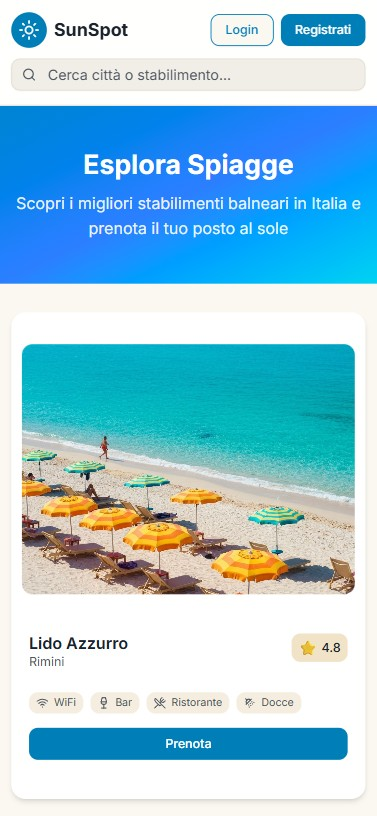
\includegraphics[width=\linewidth]{mockups/2mockup-mainPage-mobile.jpg} 
	\end{minipage}\hfill
	\begin{minipage}[b]{0.30\textwidth}
		\centering
		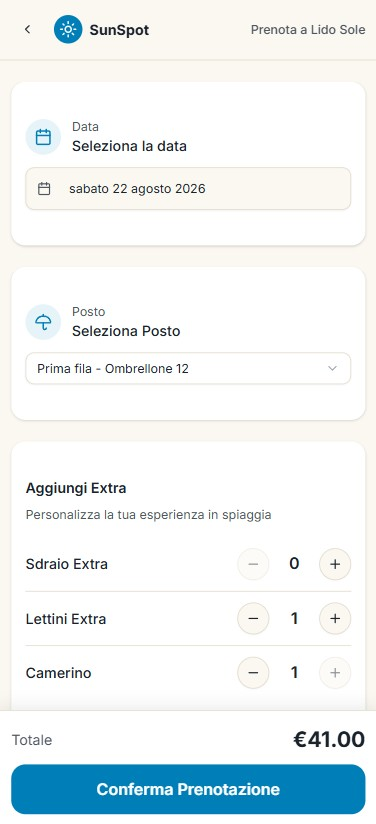
\includegraphics[width=\linewidth]{mockups/3mockup-createBooking-mobile.jpg}
	\end{minipage}\hfill
	\begin{minipage}[b]{0.30\textwidth}
		\centering
		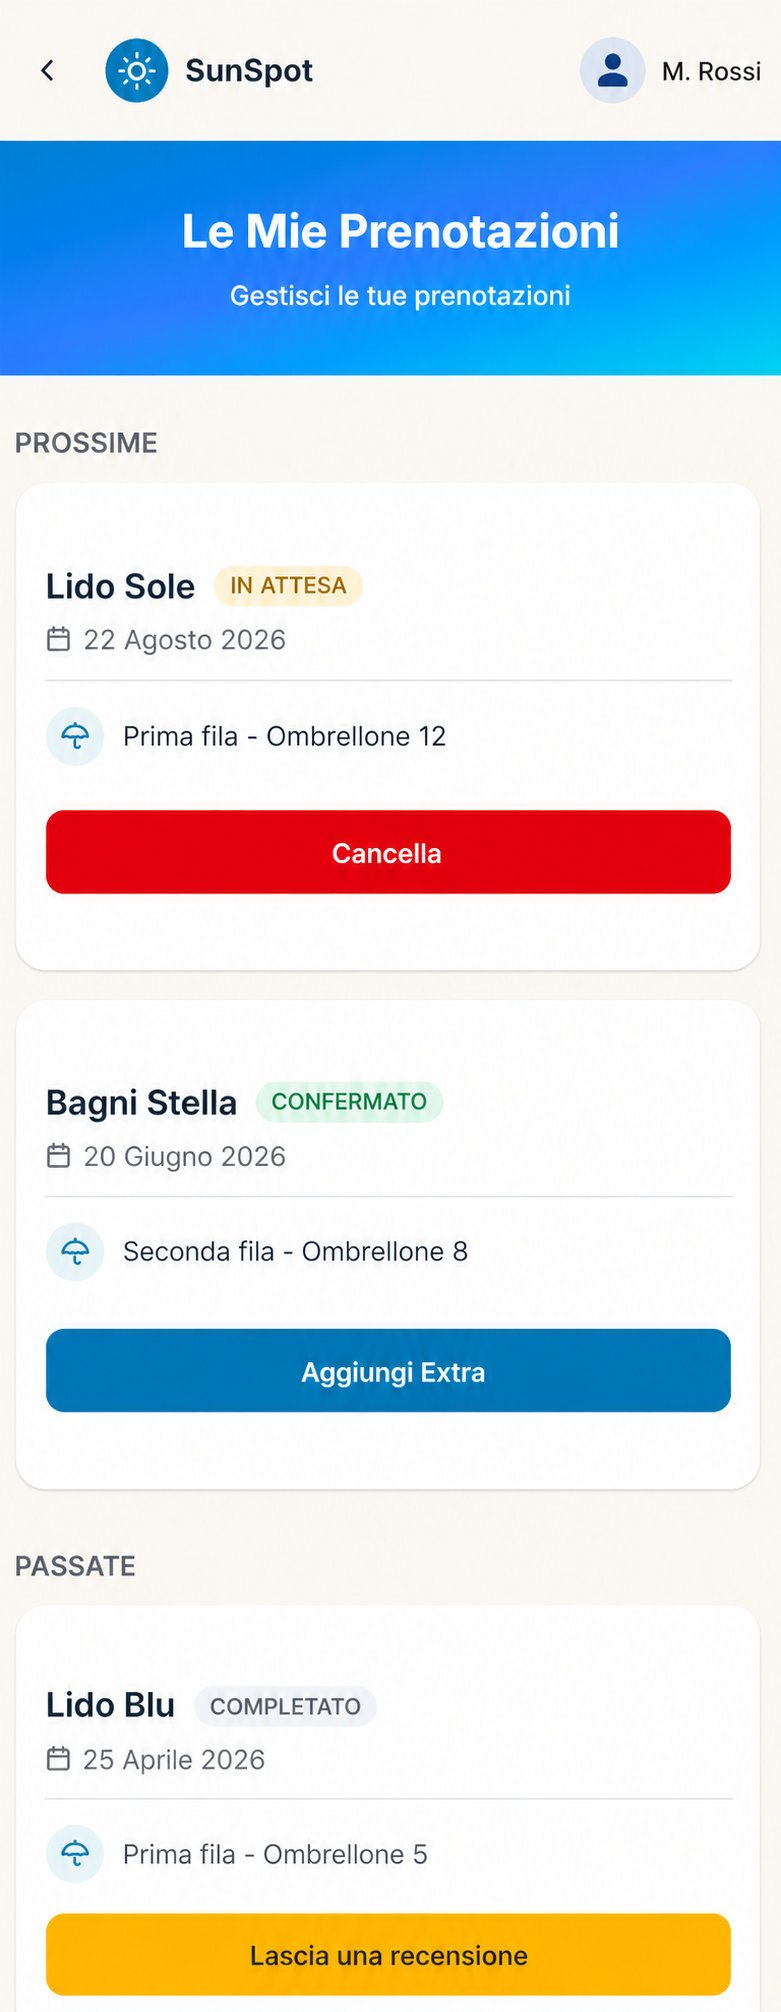
\includegraphics[width=\linewidth]{mockups/4mockup-myBookings-mobile.png}
	\end{minipage}
	
	\vspace{0.3cm}
	
	\begin{minipage}[t]{0.32\textwidth}
		\caption{\textbf{Esplora Spiagge - Mobile (UC-04):} Versione responsiva (mobile) dell'interfaccia B2C per la consultazione del catalogo spiagge da parte di Customer e Guest.}
		\label{fig:mockup2}
	\end{minipage}\hfill
	\begin{minipage}[t]{0.32\textwidth}
		\caption{\textbf{Flusso di Prenotazione (UC-05):} Interfaccia mobile per la creazione di una prenotazione. Evidenzia l'applicazione delle regole di dominio: controlli stringenti sulla capienza massima di parcheggi ed extra, e il calcolo in tempo reale del prezzo totale (tramite \textit{PriceCalculatorDomainService}).}
		\label{fig:mockup3}
	\end{minipage}\hfill
	\begin{minipage}[t]{0.32\textwidth}
		\caption{\textbf{Le Mie Prenotazioni e Recensioni (UC-06 \& UC-07):} Dashboard mobile del Customer. La UI riflette visivamente gli stati della prenotazione (\textit{PENDING} e \textit{CONFIRMED}). Viene inoltre mostrato il pulsante "Lascia una recensione", sbloccato dal backend esclusivamente per i soggiorni passati.}
		\label{fig:mockup4}
	\end{minipage}
	
\end{figure}

\begin{figure}[H]
	\centering
	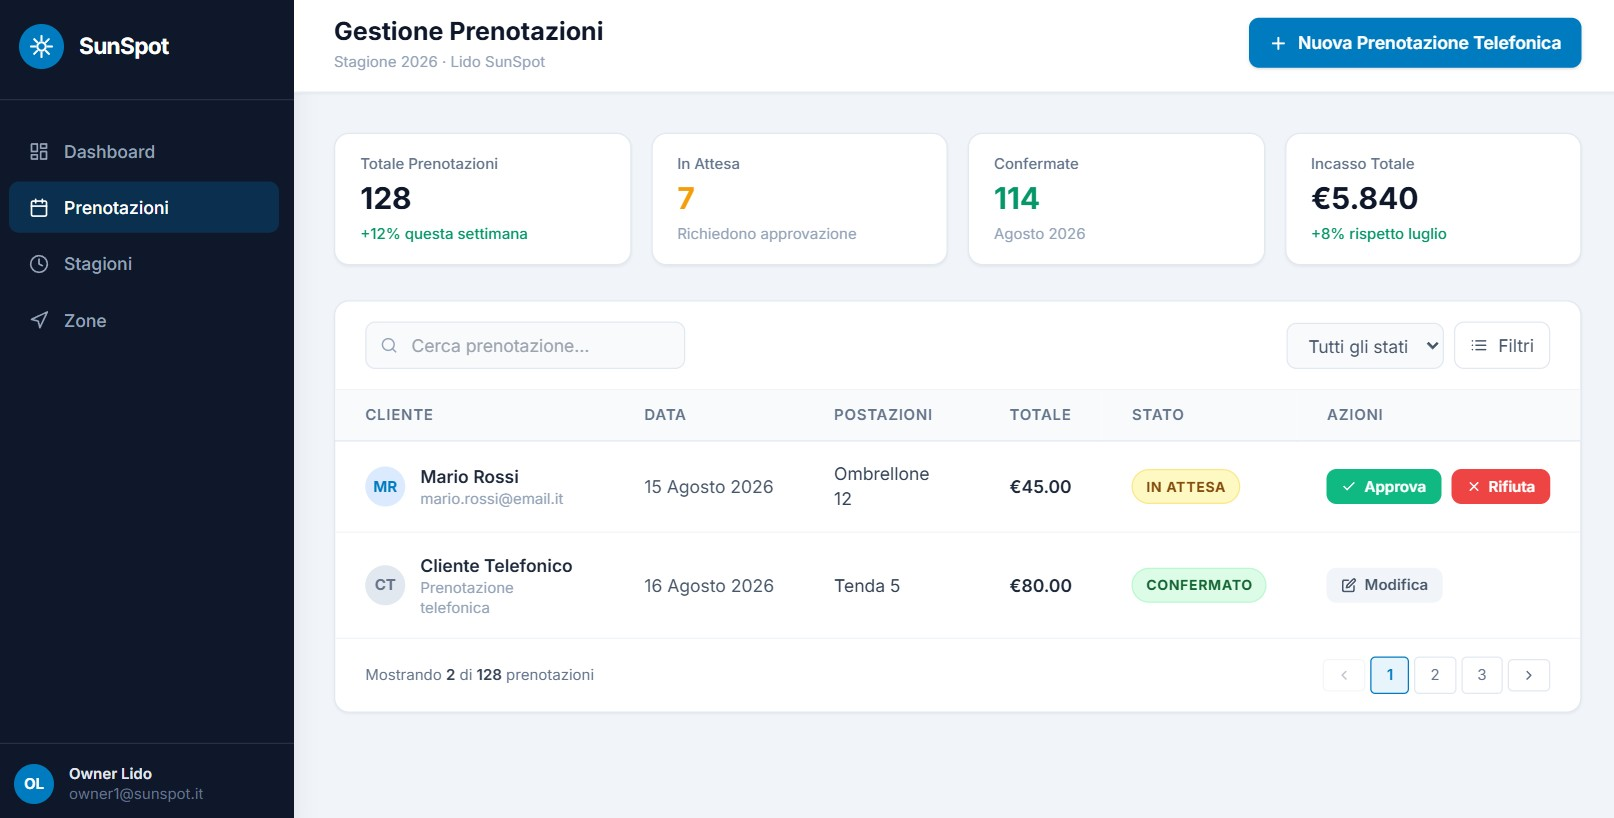
\includegraphics[width=0.9\textwidth]{mockups/5mockup-bookingMgmt-desktop.jpg}
	\caption{\textbf{Dashboard Prenotazioni Owner (UC-05 1a \& UC-06):} Interfaccia desktop B2B. Mostra la lista delle richieste in attesa con i pulsanti per l'approvazione/rifiuto e il bottone per avviare la "Prenotazione Telefonica Manuale" (che supporta dati chiamante slegati dall'ID cliente).}
	\label{fig:mockup5}
\end{figure}

\begin{figure}[H]
	\centering
	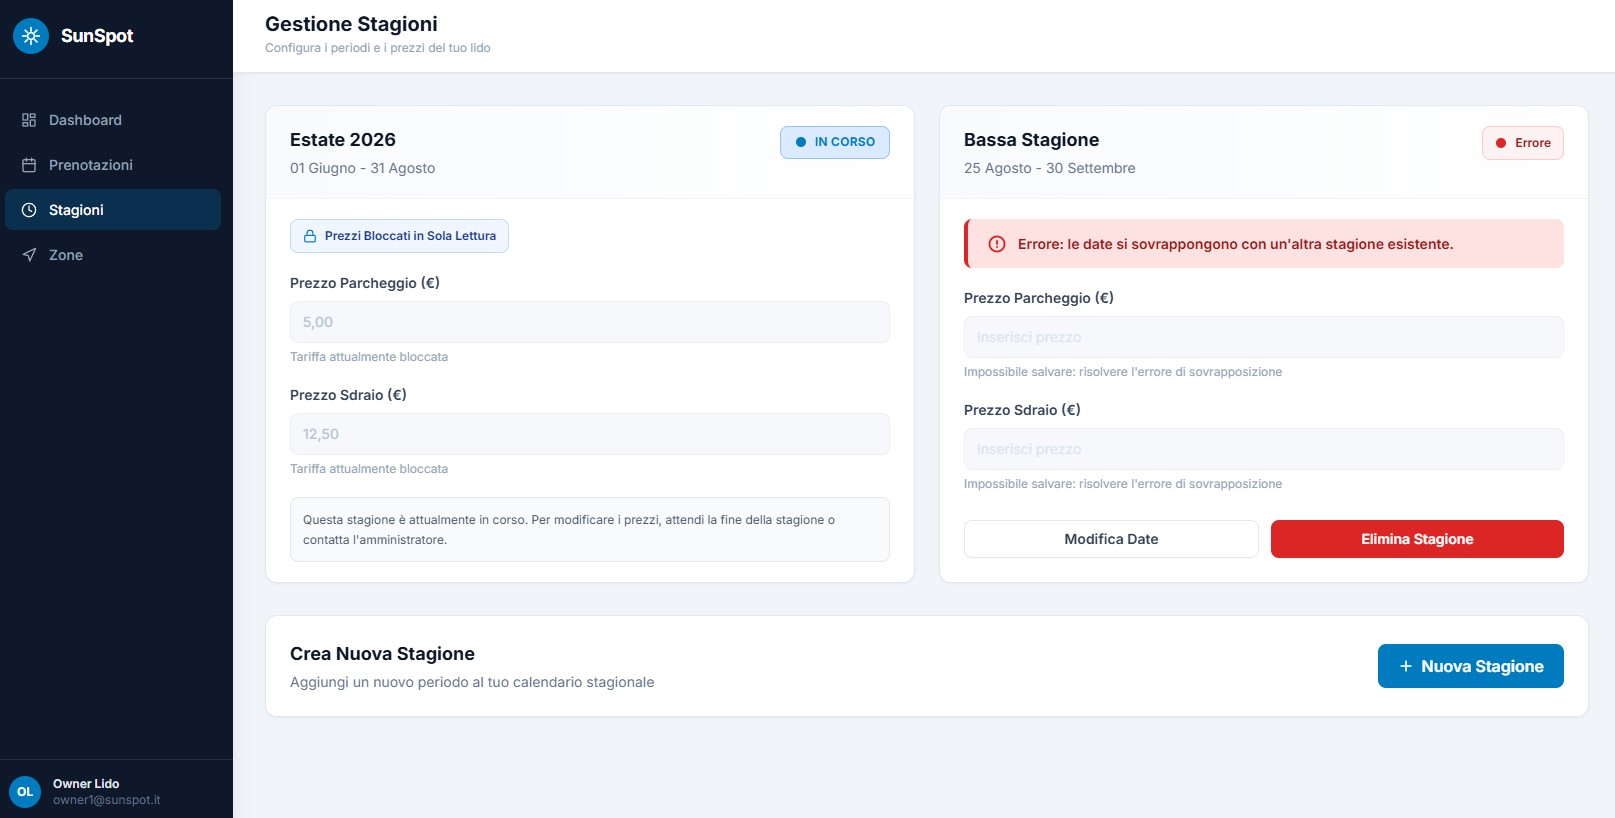
\includegraphics[width=0.9\textwidth]{mockups/6mockup-seasonsMgmt-desktop.jpg}
	\caption{\textbf{Gestione Stagioni e Prezzi (UC-14):} Il mockup dimostra l'imposizione delle regole di business del dominio: un avviso di errore per date sovrapposte (\textit{Overlap Check}) e campi prezzo resi graficamente disabilitati (Sola Lettura) per garantire l'immutabilità finanziaria.}
	\label{fig:mockup6}
\end{figure}

%\begin{figure}[H]
%	\centering
%	\includegraphics[width=0.9\textwidth]{mockups/mockup7.png}
%	\caption{\textbf{Gestione Zone e Layout (UC-15):} Strumento di mappatura della spiaggia. La figura evidenzia il blocco logico (simboleggiato dall'icona del lucchetto) applicato alle Zone già associate a una Stagione, impedendone la modifica strutturale a tutela dell'integrità dei dati.}
%	\label{fig:mockup7}
%\end{figure}

%\begin{figure}[H]
%	\centering
%	\includegraphics[width=0.9\textwidth]{mockups/mockup8.png}
%	\caption{\textbf{Dashboard di Moderazione Admin (UC-01 \& Reports):} Interfaccia desktop riservata agli Admin. Mostra la tabella delle segnalazioni evidenziando il comportamento polimorfico del Ban implementato nel backend (scelta tra \textit{App Ban} globale e \textit{Beach Ban} selettivo).}
%	\label{fig:mockup8}
%\end{figure}

\newpage

\section{Unit Testing}

\subsection{Strategia e Obiettivi del Testing}
La strategia di testing adottata per il sistema si basa sui principi della Test-Driven e Behavior-Driven validation, concentrandosi esclusivamente sui livelli \textit{Domain} e \textit{Application} dell'Architettura Esagonale. L'obiettivo principale è garantire la totale affidabilità delle regole di business e dell'orchestrazione, mantenendo i test rapidi e isolati dall'infrastruttura reale (Database).

Nello specifico, il testing è stato diviso in due macro-aree:
\begin{itemize}
	\item \textbf{Domain Layer (Test Puri):} I test sulle entità di dominio (es. \texttt{Beach}, \texttt{Booking}) e sui Value Object verificano il rispetto dei vincoli architetturali (invarianti). Garantiscono che gli oggetti non possano mai essere istanziati in stati inconsistenti (es. coordinate negative, date sovrapposte) e validano la corretta implementazione della macchina a stati (es. transizioni da PENDING a CONFIRMED) senza alcuna dipendenza esterna.
	\item \textbf{Application Layer (Test con Mock):} I test sui Service verificano la corretta orchestrazione dei casi d'uso. Utilizzando la libreria \textbf{Mockito}, le porte di uscita e il \texttt{TransactionManager} sono stati simulati (\textit{mockati}). Questo ha permesso di testare analiticamente i percorsi di successo (Happy Paths) e le barriere di sicurezza (Sad Paths), come il blocco di operazioni non autorizzate, i conflitti di capienza (Inventario/Parcheggi) e le logiche di rollback, garantendo il pieno rispetto dei requisiti utente.
\end{itemize}

\subsection{Copertura dei Test: Classi e Metodi}

\subsubsection*{Domain Layer}
I test di questo layer verificano la pura logica di business, l'integrità dei dati e i vincoli architetturali, senza alcuna dipendenza da framework o database esterni.

\begin{itemize}[leftmargin=*]
	\item \textbf{Aggregato \texttt{Beach}:}
	\begin{itemize}[nosep]
		\item \textit{Integrità e Macchina a Stati:} Validazione dei requisiti minimi per l'attivazione e blocco rigoroso delle modifiche strutturali qualora la spiaggia sia operativa (\texttt{ACTIVE}) o permanentemente chiusa (\texttt{CLOSED}).
		\item \textit{Logica Temporale (Stagioni):} Verifica dell'algoritmo di anti-sovrapposizione delle date (\textit{Overlap Check}) e dell'impossibilità di accorciare stagioni già definite.
		\item \textit{Logica Spaziale (Zone):} Test sul blocco di immutabilità che impedisce di eliminare, rinominare o alterare Zone già vincolate a una Stagione esistente.
	\end{itemize}
	
	\item \textbf{Aggregato \texttt{Booking} e \texttt{PriceCalculator}:}
	\begin{itemize}[nosep]
		\item \textit{Macchina a Stati e Sicurezza:} Transizioni di stato sicure (\textit{Pending $\rightarrow$ Confirmed $\rightarrow$ Cancelled/Rejected}) e regola di declassamento automatico: ogni modifica ad una prenotazione già confermata forza il ritorno allo stato \textit{Pending}.
		\item \textit{Integrità dei Dati:} Verifica della differenziazione tra prenotazioni di utenti registrati e chiamanti manuali (pulizia automatica del numero di telefono).
		\item \textit{Domain Service:} Test rigorosi sul \texttt{PriceCalculator} per garantire che il calcolo del totale incroci correttamente la data, la zona dello spot e il tariffario stagionale, bloccando richieste anomale (es. spot inesistenti o date fuori stagione).
	\end{itemize}
	
	\item \textbf{Gerarchia \texttt{User} (\texttt{Customer}, \texttt{Owner}, \texttt{Admin}):}
	\begin{itemize}[nosep]
		\item \textit{Validazione Ereditata:} Test astratti che garantiscono la validazione di email (formato e lunghezza), username e anagrafica per tutte le implementazioni.
		\item \textit{Comportamenti Specifici:} Gestione corretta dei flag di sicurezza (disattivazione OTP per Owner/Admin) e logica di chiusura permanente dell'account per il Customer.
	\end{itemize}
	
	\item \textbf{Moderazione (\texttt{Ban}, \texttt{Report}, \texttt{Review}):}
	\begin{itemize}[nosep]
		\item \textit{Invarianti di Dominio:} Impossibilità di auto-segnalarsi, limiti stringenti sulle valutazioni (1-5 stelle) e controlli temporali (divieto di recensioni o report nel futuro).
		\item \textit{Coerenza Polimorfica:} Verifica delle dipendenze corrette in base al tipo di Ban (un Ban globale non deve avere ID spiaggia, un Ban locale lo richiede obbligatoriamente).
	\end{itemize}
	
	\item \textbf{Value Objects e Layout (\texttt{Inventory}, \texttt{Services}, \texttt{Pricing}, \texttt{Spot}, ecc.):}
	\begin{itemize}[nosep]
		\item \textit{Contratti e Immutabilità:} Difesa assoluta contro valori matematicamente illogici (quantità o prezzi negativi).
		\item \textit{Pattern Creazionali:} Verifica dell'inizializzazione sicura tramite Static Factories (\texttt{empty()}, \texttt{none()}) e pattern Builder (incluso il costruttore copia).
		\item \textit{Copie Difensive:} Verifica che liste interne (come l'elenco di Spot in una Zona) non possano essere alterate dall'esterno una volta istanziate.
	\end{itemize}
\end{itemize}

\vspace{0.5cm} % Un po' di respiro tra Domain e Application

\subsubsection*{Application Layer (Services)}
I test di questo layer verificano la corretta orchestrazione dei flussi applicativi, l'integrazione tra aggregati distinti e l'applicazione delle regole di sicurezza, simulando le dipendenze esterne (Database e API) tramite l'uso di \textit{Mock}.

\begin{itemize}[leftmargin=*]
	\item \textbf{Gestione Spiaggia (\texttt{ManageBeachService}, \texttt{CreateBeachService}, \texttt{CloseBeachService}):}
	\begin{itemize}[nosep]
		\item \textit{Creazione e Vincoli:} Verifica del blocco architettonico della relazione 1:1 tra Owner e Beach e salvataggio automatico in stato \textit{Draft} (inattivo) in caso di configurazione parziale (UC-10).
		\item \textit{Gestione Operativa:} Test sui \textit{Delta Updates} per l'aggiornamento di Inventario e Parcheggi, garantendo che riduzioni di capienza non invalidino prenotazioni future già confermate (UC-11).
		\item \textit{Ciclo di Vita:} Verifica del processo di attivazione/disattivazione (UC-12) e chiusura irreversibile (UC-13), che garantisce l'annullamento a cascata delle prenotazioni future tramite il \texttt{BookingRepository}.
	\end{itemize}
	
	\item \textbf{Motore di Prenotazione (\texttt{CreateBookingService}, \texttt{BookingService}, \texttt{CreateManualBookingService}):}
	\begin{itemize}[nosep]
		\item \textit{Orchestrazione Sicura:} Verifica incrociata (\textit{Cross-Aggregate Validation}) prima del salvataggio: controllo disponibilità residua di parcheggi e inventario, assenza di ban attivi per l'utente, e verifica che gli spot selezionati appartengano effettivamente alla spiaggia richiesta.
		\item \textit{Prenotazioni Manuali (Owner):} Test del flusso B2B (UC-05 1a) che salta il check dell'utente (Guest calling) e impone l'approvazione automatica (stato \textit{CONFIRMED}).
		\item \textit{Vincoli Temporali:} Blocco categorico di aggiornamenti, cancellazioni o approvazioni su prenotazioni la cui data coincida con quella odierna o passata.
	\end{itemize}
	
	\item \textbf{Autenticazione e Utenze (\texttt{AuthenticationService}, \texttt{CreateUserService}, \texttt{ManageUserService}):}
	\begin{itemize}[nosep]
		\item \textit{Gateway di Sicurezza:} Test completi sul processo di Login (UC-01), che bloccano tentativi di accesso con credenziali errate, account disattivati o ban attivi (sia a livello applicativo che di struttura).
		\item \textit{Transazioni Atomiche:} Verifica del pattern \textit{Template Method} per la creazione utenti: hashing sicuro della password e rollback automatico in caso di violazione dei vincoli (es. Email/Username duplicati).
		\item \textit{Gestione Sicura Dati:} Test sulle operazioni sensibili (cambio Email o chiusura account Customer) che richiedono la ri-validazione della password attuale per essere autorizzate.
	\end{itemize}
	
	\item \textbf{Moderazione e Recensioni (\texttt{BanService}, \texttt{CreateReportService}, \texttt{ReviewService}):}
	\begin{itemize}[nosep]
		\item \textit{Polimorfismo Sanzionatorio:} Test della logica di Ban che dirama azioni differenti: un \textit{App Ban} elimina tutte le prenotazioni future (per i Customer) o chiude l'intera struttura (per gli Owner), mentre un \textit{Beach Ban} agisce solo a livello locale.
		\item \textit{Precondizioni Rigorose:} Un utente può lasciare una recensione (UC-07) o un report solo se il sistema certifica (tramite query su \texttt{BookingRepository}) un soggiorno effettivamente completato nel passato e l'assenza di provvedimenti disciplinari attivi.
		\item \textit{Prevenzione IDOR:} Verifica di sicurezza (Insecure Direct Object Reference) che impedisce a un utente di eliminare una recensione o un report non di sua proprietà.
	\end{itemize}
	
	\item \textbf{Query Services / CQRS (\texttt{BrowseBeachService}, \texttt{ManageReportService}, \texttt{ViewBeachReviewsService}):}
	\begin{itemize}[nosep]
		\item \textit{Read Models:} Test focalizzati sull'interrogazione ottimizzata dei dati, verificando la corretta aggregazione dei DTO (es. \texttt{BeachSummary}) filtrati per keyword, paginazione o stato attivo, e l'unione corretta di liste multiple (es. report ricevuti e inviati).
	\end{itemize}
\end{itemize}

\subsection{Esecuzione dei Test tramite JUnit 5 Suites}
Per facilitare l'esecuzione e l'integrazione continua (CI/CD), l'infrastruttura di test è stata organizzata utilizzando la funzionalità \textit{Test Suite} fornita da JUnit 5 (modulo \texttt{junit-platform-suite}). Sono state create tre classi orchestratrici principali:

\begin{enumerate}
	\item \textbf{\texttt{DomainTestSuite}:} Questa suite include esclusivamente i pacchetti sotto \newline \texttt{com.example.s\_balneare.domain}. È progettata per essere eseguita in pochi millisecondi. Essendo i test di dominio completamente isolati, questa suite viene utilizzata frequentemente durante lo sviluppo attivo per garantire che le modifiche non infrangano le regole matematiche o i vincoli logici degli aggregati.
	\item \textbf{\texttt{ApplicationTestSuite}:} Questa suite isola i test del pacchetto \newline \texttt{com.example.s\_balneare.application}. Richiede leggermente più memoria a causa dell'inizializzazione del framework Mockito per la simulazione delle porte di uscita, ma garantisce che tutta la logica di orchestrazione, validazione incrociata e gestione delle transazioni funzioni correttamente.
	\item \textbf{\texttt{AllTestsSuite}:} È la suite globale che esegue in sequenza sia i test di Dominio che quelli Applicativi.
\end{enumerate}

\end{document}